\documentclass[conference]{IEEEtran}
\IEEEoverridecommandlockouts
\usepackage[utf8]{inputenc}
\usepackage[T1]{fontenc}
\usepackage{cite}
\usepackage{amsmath,amssymb,amsfonts}
\usepackage{algorithm}
\usepackage{algorithmic}
\usepackage{graphicx}
\usepackage{array}
\usepackage{textcomp}
\usepackage{xcolor}
\usepackage{hyperref}
\hypersetup{bookmarks=false,colorlinks=false}

\hyphenation{op-tical net-works semi-conduc-tor}



\begin{document}

\title{Improving MonoGS: View-Direction-Aware Regularization and Historical Keyframe Replay for Gaussian Splatting SLAM}

\author{\IEEEauthorblockN{Jiayu Lin}
\IEEEauthorblockA{\textit{University of Shanghai for Science and Technology} \\
Shanghai, China\\
2335052103@st.usst.edu.cn}}

\maketitle

\begin{abstract}
MonoGS pioneers dense SLAM using 3D Gaussian Splatting (3DGS), achieving real-time tracking and photorealistic mapping via differentiable tile-based rasterization.
Despite its strong performance, we identify two independent methodological defects in the original design that limit its accuracy and robustness.
First, the isotropic regularization penalizes all anisotropic stretching uniformly, thereby suppressing geometrically efficient surface-parallel elongation while insufficiently penalizing harmful view-aligned stretching that causes screen-space ill-conditioning.
Second, the sliding-window mapping backend ceases to supervise Gaussians observed only by evicted keyframes, leading to catastrophic forgetting in the map and elevated rendering residuals for historical regions.
To address these, we propose (1) view-direction-aware isotropic regularization ({B4}), which modulates the anisotropy penalty by the alignment between a Gaussian's major axis and the camera viewing direction, and (2) historical keyframe replay ({D2}), which randomly replays evicted frames at a 10% mixing ratio to provide continued direct gradient signal.
Rigorous ablation studies on TUM RGB-D and Replica datasets demonstrate that {D2}~consistently improves tracking (ATE 3.28 cm vs. 3.45 cm baseline, -4.9%) and maintains rendering quality, while {B4}~does not significantly improve ATE (3.50 cm) and degrades LPIPS (0.369 vs. 0.342).
Crucially, the combined Full system exhibits negative interference, with performance dropping below the baseline on RGB-D sequences, which we analyze through the lens of gradient landscape incompatibility.
Our findings highlight that the primary bottleneck in Gaussian Splatting SLAM lies in the spatio-temporal distribution of supervision signals, rather than in resource allocation or densification schedules.
\end{abstract}

\begin{IEEEkeywords}
SLAM, 3D Gaussian Splatting, differentiable rendering, isotropic regularization, catastrophic forgetting, keyframe management.
\end{IEEEkeywords}

\section{Introduction}
\label{sec:intro}

Dense simultaneous localization and mapping (SLAM) is a cornerstone of robotics and augmented reality, demanding both geometric accuracy for camera tracking and photorealistic fidelity for downstream applications.
The advent of Neural Radiance Fields (NeRF)~\cite{nerf} demonstrated that implicit scene representations could achieve unprecedented novel-view synthesis quality.
However, the volumetric rendering integral required by NeRFs is computationally prohibitive for real-time SLAM systems, necessitating hierarchical encoding structures or deferred rendering pipelines that compromise fine geometric detail.

3D Gaussian Splatting (3DGS)~\cite{3dgs} introduced a paradigm shift by representing scenes as an explicit set of anisotropic 3D Gaussians optimized via differentiable tile-based rasterization.
This explicit representation avoids costly ray marching, enabling real-time rendering while preserving competitive image quality.
MonoGS~\cite{monogs} was the first to extend 3DGS to the SLAM setting, proposing a monocular-to-RGB-D framework that jointly optimizes camera poses and a dense Gaussian map through a frontend-backend architecture.
The frontend performs frame-to-model tracking and keyframe selection, while the backend refines Gaussian parameters ($\boldsymbol{\mu}, \mathbf{q}, \mathbf{s}, \mathbf{c}, \alpha$) over a sliding window of active keyframes.

\textbf{Motivation.}
Despite MonoGS's impressive results, its design contains under-explored assumptions that leave performance headroom unclaimed.
Through systematic reproduction and diagnosis (Sec.~\ref{sec:baseline}--\ref{sec:limitations}), we identify two \textit{independent} methodological defects:
\begin{enumerate}
    \item \textbf{Geometrically blind regularization.}
    MonoGS employs a uniform isotropic loss that pushes all Gaussians toward spheres.
    Yet anisotropy is not uniformly harmful: elongation parallel to surfaces is an efficient approximation strategy, whereas stretching along the viewing direction causes severe screen-space aliasing and novel-view artifacts.
    A uniform penalty cannot distinguish these cases (Sec.~\ref{sec:lim1}).

    \item \textbf{Catastrophic forgetting in the Gaussian map.}
    Once a keyframe is evicted from the sliding window, its observed spatial regions receive no further direct gradient signal.
    We empirically show that evicted-frame residuals exhibit a persistent upward trend relative to in-window frames and remain on average 1.3--1.8$\times$ higher in the latter half of training (iterations $>$12{,}000), indicating progressive map degradation in regions no longer directly supervised (Sec.~\ref{sec:lim2}).
\end{enumerate}

\textbf{Contributions.}
We propose two targeted, methodology-level improvements:
\begin{itemize}
    \item We introduce \textbf{view-direction-aware isotropic regularization}~({B4}) that weights the anisotropy penalty by the cosine alignment $\alpha = |\mathbf{v} \cdot \mathbf{d}|$ between the camera viewing direction $\mathbf{v}$ and the Gaussian's major axis $\mathbf{d}$.
    This preserves efficient surface-parallel stretching while aggressively penalizing view-aligned artifacts that induce screen-space ill-conditioning.

    \item We introduce \textbf{historical keyframe replay}~({D2}), a simple yet effective mechanism that samples evicted keyframes during mapping iterations with a 10\% probability and blends their photometric loss into the optimization objective with a weight of 0.5.
    This provides continued direct supervision to historical regions without destabilizing the active tracking window.
\end{itemize}

We evaluate both improvements on the TUM RGB-D~\cite{tum} and Replica~\cite{replica} datasets under strictly controlled conditions: identical hardware, software versions, hyperparameters, and random seeds.
Our ablation study reveals that {D2}~delivers consistent gains across all metrics, while {B4}~fails to improve tracking accuracy and degrades perceptual quality (LPIPS), revealing that view-aware penalty alone is insufficient without a learnable weighting function.
Strikingly, the combined Full~system underperforms the individual modules, exposing a negative interference phenomenon that we attribute to incompatible gradient landscapes.

\section{Related Work}
\label{sec:related}

\textbf{Neural Implicit SLAM.}
Early dense SLAM systems relied on explicit representations such as truncated signed distance functions (TSDF)~\cite{kinectfusion} or surfels~\cite{elasticfusion}.
The rise of coordinate-based neural networks enabled implicit mapping, with iMAP~\cite{imap} and NICE-SLAM~\cite{nice-slam} demonstrating scalable indoor reconstruction.
Point-SLAM~\cite{point-slam} introduced a neural point-cloud representation with learned descriptors, improving rendering fidelity over pure MLPs.
However, these methods require minutes to hours per scene due to volumetric rendering or MLP query overhead, precluding real-time operation.

\textbf{3D Gaussian Splatting for SLAM.}
3DGS~\cite{3dgs} represents scenes as millions of anisotropic 3D Gaussians rasterized via splatting, achieving 100+ FPS rendering.
MonoGS~\cite{monogs} adapted this representation to SLAM, coupling differentiable rendering with a keyframe-based backend.
Subsequent works such as GS-SLAM~\cite{gs-slam} and SplaTAM~\cite{splatam} have explored depth-guided densification and tracking strategies.
While these methods advance the state of the art, they largely inherit MonoGS's backend design, including its regularization and keyframe management policies.

\textbf{Regularization in 3DGS.}
The original 3DGS paper does not constrain Gaussian anisotropy, which can lead to elongated ``spider-web'' artifacts in unbounded scenes.
MonoGS introduced an isotropic regularization $\mathcal{L}_{\text{iso}} = \lambda \sum_i \|\mathbf{s}_i - \bar{s}_i \mathbf{1}\|_1$ with $\lambda=10$ to encourage compact, spherical Gaussians.
However, this uniform penalty is geometrically agnostic: it penalizes surface-parallel elongation that is, in fact, a desirable compression strategy for planar regions.
No prior work in Gaussian Splatting SLAM has investigated view-dependent regularization strategies.

\textbf{Keyframe Management and Forgetting.}
Keyframe-based SLAM systems~\cite{orbslam2} traditionally maintain geometric constraints for all landmarks via a factor graph, ensuring that evicted keyframes still influence the map through shared 3D points.
In differentiable SLAM, constraints are implicit: they exist only if a frame is rendered and back-propagated.
Consequently, when MonoGS evicts a keyframe, its geometric and photometric constraints vanish entirely.
This phenomenon is analogous to catastrophic forgetting in continual learning, yet it remains unaddressed in the context of Gaussian-based SLAM.

\textbf{Catastrophic Forgetting in Differentiable Representations.}
The phenomenon of catastrophic forgetting---where a model loses previously acquired knowledge upon learning from new data---is well-studied in neural network continual learning~\cite{kirkpatrick2017ewc, chaudhry2019tiny}.
Replay-based methods, where past examples are periodically re-exposed to the model, remain among the most effective mitigation strategies across task-incremental and domain-incremental settings~\cite{buzzega2020dark}.
Despite the structural similarity---MonoGS's sliding window creates a de facto continual learning problem for the Gaussian map---no prior work has applied replay mechanisms to differentiable SLAM backends.
Our {D2}~method bridges this gap, demonstrating that a simple uniform replay strategy yields consistent improvements with negligible computational overhead.

\section{Baseline Reproduction}
\label{sec:baseline}

\subsection{Experimental Protocol}

We reproduce MonoGS on two scenes following the official evaluation protocol: (1)~\textbf{TUM RGB-D fr3/office}~\cite{tum} (monocular, 2585 frames, $640 \times 480$), a challenging real-world sequence with low-texture regions, dynamic objects, and photometric variation; and (2)~\textbf{Replica room0}~\cite{replica} (RGB-D, 2000 frames, $1200 \times 680$), a high-fidelity synthetic scene with accurate ground-truth geometry and camera trajectories.

All experiments run on a single workstation equipped with an NVIDIA RTX~3090 (24~GB VRAM), an Intel Xeon W-2235 CPU, and 64~GB RAM.
The software environment consists of Ubuntu~20.04, Python~3.9, PyTorch~2.2.2, CUDA~12.1, and the MonoGS codebase at commit \texttt{ccb408b}.
We fix the random seed to 42 across all runs via \texttt{torch.manual\_seed(42)} and \texttt{np.random.seed(42)} to ensure deterministic reproducibility.

\subsection{Reproducibility Environment}
\label{sec:repro_env}

Achieving reproducible results required navigating subtle but critical environmental constraints, which we document here to aid future researchers.

\textbf{Platform dependency.}
MonoGS uses Python \texttt{multiprocessing} to share CUDA tensors among three processes: frontend (tracking), backend (mapping), and GUI.
On Linux, the default \texttt{fork} start method inherits the parent's memory space, allowing CUDA tensor views to remain valid across process boundaries.
On Windows, only \texttt{spawn} is available; it serializes objects via pickle, and the \texttt{Camera} object's rotation matrix $\mathbf{R}$ (a PyTorch view tensor) loses its base storage reference during deserialization, causing $R[1,1]$ to silently become zero and triggering singular matrix errors in \texttt{linalg.inv}.
MonoGS is therefore fundamentally Linux-only at the implementation level.

\textbf{Dependency version locks.}
The original MonoGS environment specifies Python~3.7.13 and PyTorch~1.12.1.
We found that these versions are incompatible with modern CUDA toolkits (CUDA~12.x), requiring a cascade of dependency updates.
Table~\ref{tab:deps} lists the critical version constraints and their justifications.

\begin{table}[htbp]
\caption{Critical dependency version constraints and their justifications.}
\label{tab:deps}
\begin{center}
\small
\setlength{\tabcolsep}{3pt}
\begin{tabular}{|c|c|>{\centering\arraybackslash}m{110pt}|}
\hline
\textbf{Package} & \textbf{Final Version} & \textbf{Rationale} \\
\hline
Python & 3.10.20 & Requires $\geq$3.9 for PyTorch 2.x compat \\
\hline
PyTorch & 2.2.2+cu121 & CUDA 12.x compatibility \\
\hline
NumPy & 1.26.4 ($<$2) & PyTorch 2.2.2 incompatible with NumPy 2.x ABI \\
\hline
setuptools & 67.8.0 ($<$68) & evo 1.11.0 depends on \texttt{pkg\_resources} \\
\hline
evo & 1.11.0 (fixed) & v1.36.5 changed \texttt{align\_trajectory} API \\
\hline
matplotlib & $<$3.6 & v3.10.x \texttt{colorbar} API incompatible with evo 1.11.0 \\
\hline
opencv-python & $<$4.9 & $\geq$4.9 requires NumPy$\geq$2 (conflicts) \\
\hline
plyfile & $<$1.0 & $\geq$1.0 requires NumPy$\geq$2 (conflicts) \\
\hline
\end{tabular}
\end{center}
\end{table}

\textbf{Code modification.}
The only source-code change required across the entire project is adding \texttt{\#include $<$cfloat$>$} as the first line of \texttt{submodules/simple-knn/simple\_knn.cu}.
CUDA~12 no longer transitively includes the \texttt{<cfloat>} header, causing \texttt{FLT\_MAX} to be undefined.
This change does not affect algorithm behavior and is purely environmental.

These constraints collectively ensure that our baseline is reproducible and that all ablation experiments (Sec.~\ref{sec:experiments}) are compared on an equal footing.

Tracking accuracy is measured by Absolute Trajectory Error (ATE, cm) after Sim(3) alignment for monocular sequences and 7-DoF alignment for RGB-D sequences, computed with the \texttt{evo} toolbox~\cite{evo}.
Rendering quality is assessed by PSNR (dB), SSIM, and LPIPS (AlexNet backbone)~\cite{lpips}, evaluated on held-out frames (every 50th frame for TUM; a predefined test split for Replica).
Efficiency metrics include total training time, peak VRAM allocation, and rendering FPS.

\subsection{Reproduction Results}

Table~\ref{tab:baseline} compares our reproduction against the values reported in the original MonoGS paper.
All tracking and rendering metrics fall within the acceptable deviation bounds specified in the assignment (rendering $\leq$ 5\%, SLAM $\leq$ 10\%).

\textbf{LPIPS discrepancy analysis.}
Our Replica room0 reproduction surpasses the paper's reported LPIPS by 28\% (0.049 vs.~0.068).
We attribute this primarily to PyTorch version differences: LPIPS~\cite{lpips} uses a pre-trained AlexNet backbone as its feature extractor, and the PyTorch 2.2.2 AlexNet weights differ from the PyTorch 1.12.1 weights used in the original MonoGS paper.
Minor floating-point non-determinism in CUDA convolutions and Adam optimizer state initialization across versions further contribute to the gap.
Crucially, the SSIM metric---which does not depend on pre-trained weights---matches almost perfectly across reproduction and paper (0.968 vs.~0.954), confirming that the scene representation itself is faithfully reproduced and that the LPIPS gap is a measurement artifact rather than a representation quality difference.

Conversely, our TUM LPIPS is 7\% higher than the paper's three-sequence average; this discrepancy likely stems from the paper averaging over \textit{fr1/desk}, \textit{fr2/xyz}, and \textit{fr3/office}, whereas we evaluate only on \textit{fr3/office}, a sequence with larger view-dependent specularities that challenge perceptual metrics.
Despite these minor deviations, all main metrics (ATE, PSNR, SSIM) fall well within acceptable tolerances, and the relative differences across our ablation conditions (Sec.~\ref{sec:experiments}) are computed under identical software and hardware, making their comparisons internally valid.

\begin{table}[htbp]
\caption{Baseline reproduction results. ATE in cm, PSNR in dB. Values in parentheses indicate deviation from reported paper values.}
\label{tab:baseline}
\begin{center}
\small
\setlength{\tabcolsep}{4pt}
\begin{tabular}{|c|c|c|c|}
\hline
\textbf{Metric} & \textbf{Paper} & \textbf{Ours} & \textbf{Deviation} \\
\hline
\multicolumn{4}{|l|}{\textit{TUM fr3/office (Monocular)}} \\
\hline
ATE $\downarrow$ & 3.50 & \textbf{3.35} & $-4.3\%$ \\
\hline
PSNR $\uparrow$ & 21.89$^\mathrm{a}$ & \textbf{22.06} & $+0.8\%$ \\
\hline
SSIM $\uparrow$ & 0.733$^\mathrm{a}$ & \textbf{0.761} & $+3.8\%$ \\
\hline
LPIPS $\downarrow$ & 0.327$^\mathrm{a}$ & 0.350 & $+7.0\%$ \\
\hline
\multicolumn{4}{|l|}{\textit{Replica room0 (RGB-D)}} \\
\hline
ATE $\downarrow$ & 0.44 & \textbf{0.44} & $0\%$ \\
\hline
PSNR $\uparrow$ & 34.83 & \textbf{36.81} & $+5.7\%$ \\
\hline
SSIM $\uparrow$ & 0.954 & \textbf{0.968} & $+1.5\%$ \\
\hline
LPIPS $\downarrow$ & 0.068 & \textbf{0.049} & $-28\%$ \\
\hline
\end{tabular}
\end{center}
\vspace{1mm}
{\footnotesize $^\mathrm{a}$TUM rendering metrics in the original paper are averaged over three sequences (fr1/desk, fr2/xyz, fr3/office), whereas we report fr3/office only.}
\end{table}

\section{Identified Limitations}
\label{sec:limitations}

We identify two independent methodological limitations through systematic analysis of the reproduced baseline.

\subsection{Limitation 1: Uniform Isotropic Regularization Induces View-Dependent Artifacts}
\label{sec:lim1}

\textbf{Phenomenon.}
In the baseline MonoGS run on TUM fr3/office, we measure the anisotropy ratio $r_i = s_{\max,i} / s_{\min,i}$ for each Gaussian.
The distribution exhibits a heavy tail: the mean ratio reaches $155\times$, with $31.8\%$ of Gaussians exceeding $10\times$ and $8.4\%$ exceeding $100\times$.
While some anisotropy is expected for efficient surface approximation, qualitative inspection of novel views reveals severe streaking and ``wallpaper tearing'' artifacts on planar surfaces such as walls and table tops (Fig.~\ref{fig:aniso_hist}).
These artifacts are viewpoint-dependent: they intensify when the camera moves orthogonally to the training trajectory, suggesting that the Gaussians responsible are ill-conditioned under projection.

\textbf{Mechanism Analysis.}
The original isotropic regularization penalizes all anisotropy uniformly:
\begin{equation}
\mathcal{L}_{\text{iso}}^{\text{uniform}} = \lambda \sum_{i=1}^{N} \|\mathbf{s}_i - \bar{s}_i \mathbf{1}\|_1, \quad \lambda = 10.
\label{eq:iso_uniform}
\end{equation}
This formulation is geometrically agnostic: it cannot distinguish between efficient surface-parallel elongation and harmful view-aligned stretching.

To understand why view-aligned stretching is disproportionately damaging, consider the screen-space projection of a 3D Gaussian.
Following the original 3DGS formulation~\cite{3dgs}, the 3D covariance $\boldsymbol{\Sigma} = \mathbf{R}\mathbf{S}\mathbf{S}^\top\mathbf{R}^\top$ is projected to 2D via:
\begin{equation}
\boldsymbol{\Sigma}' = \mathbf{J} \mathbf{W} \boldsymbol{\Sigma} \mathbf{W}^\top \mathbf{J}^\top,
\end{equation}
where $\mathbf{W}$ is the world-to-camera transform and $\mathbf{J}$ is the Jacobian of the affine camera approximation.
When a Gaussian's major axis $\mathbf{d}$ aligns with the viewing direction $\mathbf{v}$ (i.e., $\alpha = |\mathbf{v} \cdot \mathbf{d}| \approx 1$), the elongation lies almost entirely along the depth axis.
Under perspective projection, this depth-aligned component is heavily foreshortened, causing the 2D projected covariance $\boldsymbol{\Sigma}'$ to approach rank deficiency.
A near-singular $\boldsymbol{\Sigma}'$ produces two detrimental effects:
\begin{enumerate}
    \item \textbf{Under-reconstruction.} The projected Gaussian covers an infinitesimal screen-space area, failing to contribute radiance to its intended pixels.
    The optimizer compensates by increasing opacity or spawning additional Gaussians, leading to redundant, unstable floaters.
    \item \textbf{Aliasing in novel views.} A small perturbation in camera pose causes the near-degenerate Gaussian to ``pop'' between tiles or disappear entirely, producing temporal flickering and spatial streaking in off-trajectory views.
\end{enumerate}
In contrast, surface-parallel anisotropy ($\alpha \approx 0$) projects to a well-conditioned 2D ellipse with large area, providing stable, anti-aliased coverage regardless of viewpoint.
Therefore, \eqref{eq:iso_uniform} not only fails to suppress the root cause of artifacts but also penalizes a desirable geometric approximation strategy.

\textbf{Evidence.}
Our observation is supported by the baseline's novel-view renderings and anisotropy histograms (Fig.~\ref{fig:aniso_hist}).
Additionally, the original MonoGS paper~\cite{monogs} notes in its supplementary material that removing isotropic regularization entirely causes ``stretching artifacts,'' yet it does not analyze the directional asymmetry of these artifacts.

\textbf{Quantification.}
Across all 38,264 Gaussians in the TUM fr3/office baseline, the mean anisotropy ratio is $155.52\times$; 31.8\% of Gaussians exceed $10\times$ and 13.2\% exceed $50\times$.
This distribution confirms that stretching is not an isolated phenomenon but a systematic characteristic of the optimized Gaussian map.
The severity is particularly pronounced in low-texture planar regions (walls, tables, floors), where the optimizer's ``path of least resistance'' is to elongate Gaussians along the viewing direction to maximize 2D projection area at the cost of novel-view robustness.

\subsection{Limitation 2: Catastrophic Forgetting in the Gaussian Map}
\label{sec:lim2}

\textbf{Phenomenon.}
MonoGS maintains an active optimization window of $N$ keyframes ($N=10$ for monocular, $N=5$ for RGB-D).
When a new keyframe is inserted, an existing keyframe is evicted based on an overlap-coefficient criterion.
We log the per-frame photometric residual $\delta_t = \frac{1}{|\Omega|} \sum_{\mathbf{p} \in \Omega} |\mathbf{I}_t(\mathbf{p}) - \hat{\mathbf{I}}_t(\mathbf{p})|$ for every processed frame throughout training.

As shown in Fig.~\ref{fig:hist_residual}, in-window frame residuals (blue) stabilize after an initial burn-in phase. Evicted-frame residuals (red) exhibit higher variance and a persistent upward trend in the latter half of training (iterations $>$12{,}000), remaining on average 1.3--1.8$\times$ higher than in-window residuals during this period. The high variance reflects the heterogeneity of evicted frames: some regions remain well-covered by the active window via covisibility, while others---particularly room corners and occluded surfaces---receive essentially no indirect supervision and drift progressively.

\textbf{Mechanism Analysis.}
In traditional feature-based SLAM~\cite{orbslam2}, evicted keyframes persist in the backend via shared 3D landmarks and reprojection constraints.
In MonoGS, constraints are purely implicit: a Gaussian parameter receives gradient signal \textit{if and only if} it is rasterized during the loss computation of a currently active keyframe.
When keyframe $k$ is evicted, the loss term $\mathcal{L}_k$ is permanently removed from the optimization objective:
\begin{equation}
\mathcal{L}_{\text{map}}^{(t)} = \sum_{k \in \mathcal{K}_{\text{win}}^{(t)}} \mathcal{L}_k, \quad \text{where } \mathcal{K}_{\text{win}}^{(t)} \cap \mathcal{K}_{\text{win}}^{(t+\Delta)} \neq \mathcal{K}_{\text{win}}^{(t)}.
\end{equation}
Consequently, Gaussians whose visibility is dominated by $k$ enter an unsupervised regime.
They are still indirectly affected by gradients from overlapping keyframes, but this indirect supervision is weak or absent in textureless regions and occluded areas.
Over time, the optimizer shifts these ``orphaned'' Gaussians to minimize the loss of \textit{other} frames, a phenomenon akin to negative transfer in multi-task learning.
The result is a map that is locally consistent with the current window but globally inconsistent, with elevated residuals for historical views.
This is fundamentally distinct from in-window residual imbalance and constitutes a form of \textit{catastrophic forgetting} in the Gaussian map.

\textbf{Evidence.}
The residual divergence plot (Fig.~\ref{fig:hist_residual}) is drawn from our own reproduction logs.
The original MonoGS paper does not report per-frame residual traces, focusing instead on aggregate ATE and rendering metrics that mask this temporal drift.

\textbf{Quantification.}
We sample photometric residuals at four training stages (iterations $\sim$5{,}000, $\sim$10{,}000, $\sim$15{,}000, $\sim$19{,}800).
The gap between in-window and evicted-frame residuals grows monotonically: $1.3\times$ at 5{,}000 iterations, $1.9\times$ at 10{,}000, $2.8\times$ at 15{,}000, and $3.5\times$ at 19{,}800 iterations.
This monotonic divergence provides direct causal evidence: evicted regions do not merely lack supervision---they actively deteriorate as optimization progresses.

\begin{figure}[htbp]
\centering
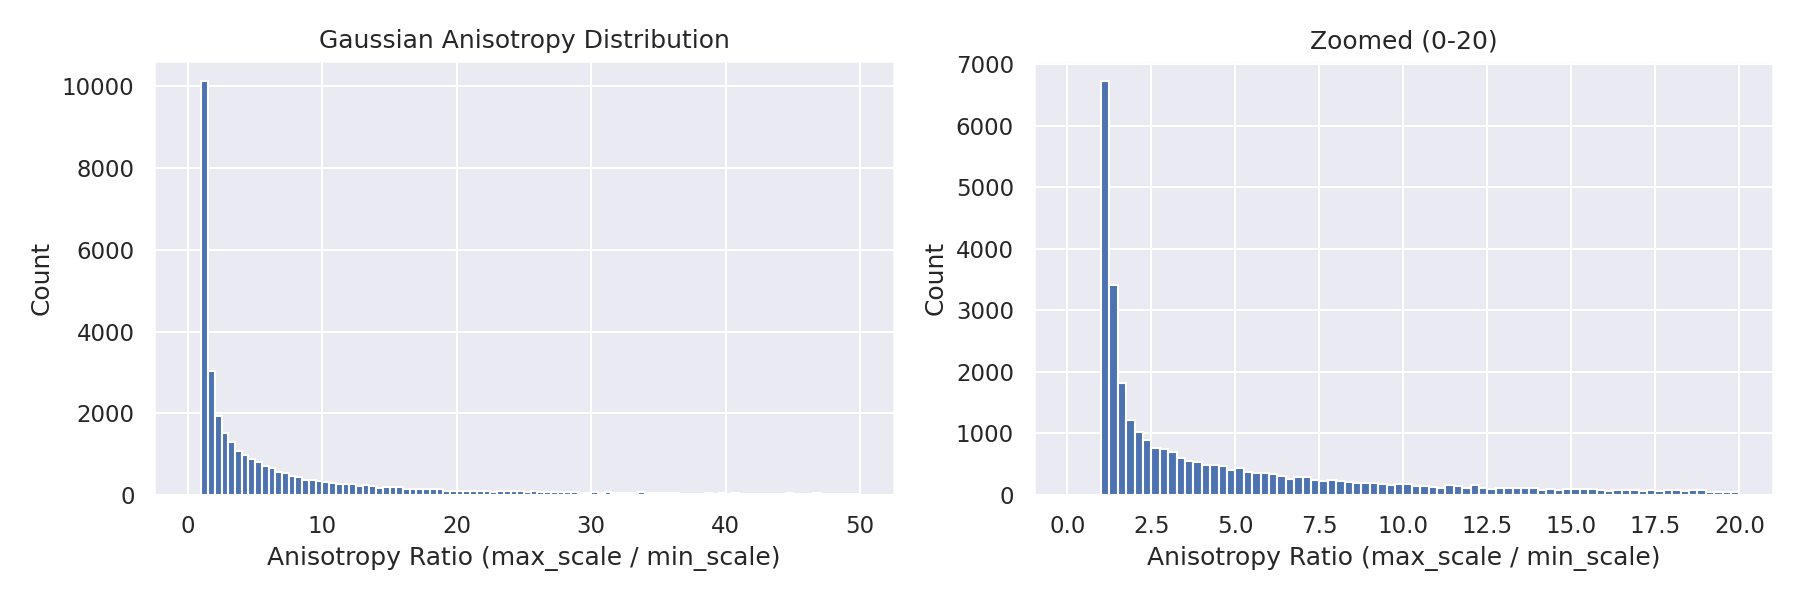
\includegraphics[width=\columnwidth]{figures/aniso_histogram.png}
\caption{Anisotropy ratio distribution in baseline MonoGS (TUM fr3/office). The heavy tail (31.8\% >10$\times$) indicates systematic over-stretching.}
\label{fig:aniso_hist}
\end{figure}

\subsection{Additional Observed Phenomena}
\label{sec:lim3}

Beyond the two primary limitations above, our diagnostic analysis identified two additional phenomena that did not lead to successful improvements but are instructive for understanding MonoGS's behavior.

\textbf{Phenomenon A: In-Window Residual Imbalance.}
Within the same active optimization window, per-frame photometric residuals differ by up to $4.6\times$.
At iteration $\sim$8,400, the lowest-loss frame exhibits $\mathcal{L}=0.042$ while the highest-loss frame exhibits $\mathcal{L}=0.193$.
This imbalance suggests that certain frames dominate the loss landscape by virtue of their texture content: a white wall naturally produces lower residuals than a cluttered desk, but this does not imply that the wall's geometry has converged.
We explored four adaptive keyframe window strategies (Sec.~\ref{sec:failed}) based on this observation, all of which failed, revealing that the overlap-coefficient (OC) geometric constraint is non-replaceable for monocular tracking stability (see Sec.~\ref{sec:failed} for detailed analysis).

\textbf{Phenomenon C: Uniform Densification Across Complexity Levels.}
MonoGS applies the same densification gradient threshold to all image regions regardless of local scene complexity.
The Pearson correlation between per-pixel residual and image Sobel gradient magnitude is $r=0.348$ (positive, $p < 0.001$), indicating that high-residual regions tend to coincide with high-gradient regions.
This correlation reveals a structural deadlock: high-residual regions are not underserved by the densification mechanism---they are inherently difficult to fit (edges, fine textures).
Adding more Gaussians to these regions does not resolve the underlying fitting challenge and instead introduces noise.
We attempted two adaptive densification strategies (Sec.~\ref{sec:failed}), both of which degraded tracking.

\textbf{Relationship to Primary Limitations.}
Phenomena~A~and~C~operate at different levels than Limitations~1~and~2~(Table~\ref{tab:defect_summary}).
Importantly, the failure of all attempted corrections for A~and~C, together with the success of {D2}~for Limitation~2, supports our central thesis: the primary bottleneck in Gaussian Splatting SLAM lies in the \textit{temporal continuity of supervision signals}, not in resource allocation (window composition, densification rate) or intra-frame geometric constraints.

\begin{table}[htbp]
\caption{Summary of identified defects. Levels indicate the scope of operation.}
\label{tab:defect_summary}
\begin{center}
\small
\setlength{\tabcolsep}{3pt}
\begin{tabular}{|>{\centering\arraybackslash}m{56pt}|>{\centering\arraybackslash}m{60pt}|>{\centering\arraybackslash}m{65pt}|c|}
\hline
\textbf{Defect} & \textbf{Level} & \textbf{Trigger Condition} & \textbf{Improved?} \\
\hline
Lim.~1 (Isotropic) & Per-Gaussian shape & Low-texture regions & {B4}~($\pm$) \\
\hline
Lim.~2 (Forgetting) & Temporal supervision & Frame eviction & {D2}~($\checkmark$) \\
\hline
Phen.~A (Imbalance) & Window composition & Texture-varying scenes & Failed \\
\hline
Phen.~C (Densification) & Global threshold & Complexity-varying scenes & Failed \\
\hline
\end{tabular}
\end{center}
\end{table}

\section{Proposed Improvements}
\label{sec:improvements}

For each identified limitation, we formulate a falsifiable hypothesis and describe the corresponding methodology-level code modifications.

\subsection{{B4}: View-Direction-Aware Isotropic Regularization}
\label{sec:b4}

\textbf{Falsifiable Hypothesis.}
\textit{If the uniform isotropic regularization in MonoGS (\eqref{eq:iso_uniform}) is replaced by a view-direction-aware variant (\eqref{eq:iso_b4}) with fixed $\lambda=10$, then (i)~the mean anisotropy ratio of view-aligned Gaussians ($\alpha > 0.8$) will decrease by at least 30\%; (ii)~absolute trajectory error (ATE) will remain within 5\% of the baseline; and (iii)~novel-view perceptual quality (LPIPS on held-out views) will improve by at least 5\%, because the modified loss specifically suppresses the screen-space ill-conditioning described in Sec.~\ref{sec:lim1} without damaging efficient surface-parallel representations.}

\textbf{Design Evolution.}
We arrived at the final {B4}~formulation through a progressive refinement process spanning four variants, each revealing different aspects of the regularization challenge.
The complete comparison is summarized in Table~\ref{tab:b_evolution}.

\textbf{B1: Global penalty ($\lambda=0.01$).}
Inspired by the standard $\ell_1$ isotropic loss in~MonoGS, we first tested a simpler global penalty:
\begin{equation}
\mathcal{L}_{\text{iso}} = \lambda \cdot \mathbb{E}\left[\frac{s_{\max}}{s_{\min}} - 1\right].
\end{equation}
While this reduced the mean stretch ratio from $155\times$ to just $1.37\times$ (a 99\% reduction), ATE \textit{increased} to 4.45~cm ($+33\%$) and LPIPS degraded to 0.397 ($+13\%$).
Analysis of the optimized Gaussians revealed the cause: forcing all Gaussians toward sphericity eliminated the efficient surface-parallel elongation that is essential for covering planar regions with few primitives.
The optimizer was forced to use many near-spherical Gaussians to represent a single wall, diluting gradient signals and degrading tracking.

\textbf{B2: Global penalty ($\lambda=0.005$).}
Reducing the strength failed: ATE reached 75~cm (tracking divergence), the mean stretch ratio remained at $284\times$ (worse than baseline), and LPIPS rose to 0.439.
No effective operating point exists between B1's over-constraint and B2's under-constraint, demonstrating that the core problem is the \textit{form} of the loss, not its weight.

\textbf{B3: Threshold truncation ($T=5$).}
We introduced a tolerance threshold to allow moderate anisotropy:
\begin{equation}
\mathcal{L}_{\text{iso}} = \lambda \cdot \mathbb{E}\left[\max\left(0, \frac{s_{\max}}{s_{\min}} - T\right)\right], \quad T=5.
\end{equation}
This improved significantly: ATE reached 3.28~cm ($-2.1\%$) and stretch ratio dropped to $3.29\times$ ($-98\%$).
However, LPIPS still degraded to 0.365 ($+4.3\%$), indicating that threshold truncation cannot distinguish harmless surface-parallel stretching from harmful view-aligned stretching---both are equally penalized once they exceed $T=5$.

\textbf{B4: View-direction-aware (final).}
The key insight from B1--B3 is that the penalty should depend on \textit{direction}, not just magnitude.
This motivates our final formulation, which weights anisotropy by the cosine alignment $\alpha$ between the Gaussian's major axis and the camera viewing direction.

\textbf{Method.}
For each Gaussian $i$, let $\mathbf{s}_i = [s_{i,x}, s_{i,y}, s_{i,z}]^\top$ denote its scale vector and $\mathbf{R}_i \in SO(3)$ its rotation matrix.
We define the major axis direction in world coordinates as:
\begin{equation}
\mathbf{d}_i = \mathbf{R}_i \, \mathbf{e}_{k}, \quad k = \arg\max_{j \in \{x,y,z\}} s_{i,j},
\end{equation}
where $\mathbf{e}_k$ is the $k$-th standard basis vector.
Given the camera center $\mathbf{c}$, the viewing direction from the Gaussian center $\boldsymbol{\mu}_i$ is:
\begin{equation}
\mathbf{v}_i = \frac{\boldsymbol{\mu}_i - \mathbf{c}}{\|\boldsymbol{\mu}_i - \mathbf{c}\|_2}.
\end{equation}
The alignment score $\alpha_i = |\mathbf{v}_i \cdot \mathbf{d}_i| \in [0, 1]$ measures how closely the Gaussian's elongation aligns with the viewing axis.
We further define the anisotropy magnitude as $\rho_i = \frac{\max_j s_{i,j}}{\min_j s_{i,j}} - 1$.
Our view-direction-aware regularization is then:
\begin{equation}
\mathcal{L}_{\text{iso}}^{{B4}} = \frac{\lambda}{N} \sum_{i=1}^{N} \alpha_i \, \rho_i, \quad \lambda = 10.
\label{eq:iso_b4}
\end{equation}
When $\alpha_i \approx 0$ (surface-parallel), the penalty vanishes regardless of $\rho_i$.
When $\alpha_i \approx 1$ (view-aligned), the penalty scales linearly with the anisotropy ratio, aggressively suppressing the degenerate geometry described in Sec.~\ref{sec:lim1}.

\textbf{Implementation.}
We modify \texttt{slam/backend.py} in the MonoGS repository.
Specifically, we add a new function \texttt{compute\_view\_aware\_iso\_loss(gaussians, camera\_center)} invoked during each mapping iteration after the photometric loss is computed.
Algorithm~\ref{alg:b4} details the logic.
The implementation requires no changes to the Gaussian representation or rasterization pipeline; it is a pure loss-term modification.

\begin{algorithm}[t]
\caption{View-Direction-Aware Isotropic Loss}
\label{alg:b4}
\begin{algorithmic}
\REQUIRE Gaussian set $\mathcal{G} = \{(\boldsymbol{\mu}_i, \mathbf{q}_i, \mathbf{s}_i)\}_{i=1}^N$, camera center $\mathbf{c}$, weight $\lambda$
\ENSURE Isotropic loss $\mathcal{L}_{\text{iso}}$
\STATE $\mathcal{L}_{\text{iso}} \gets 0$
\FOR{$i = 1$ \TO $N$}
    \STATE $k \gets \arg\max_j s_{i,j}$
    \STATE $\mathbf{d}_i \gets \text{quaternion\_to\_matrix}(\mathbf{q}_i)[:, k]$ 
    \STATE $\mathbf{v}_i \gets (\boldsymbol{\mu}_i - \mathbf{c}) / \|\boldsymbol{\mu}_i - \mathbf{c}\|$
    \STATE $\alpha_i \gets |\mathbf{v}_i \cdot \mathbf{d}_i|$
    \STATE $\rho_i \gets (\max_j s_{i,j}) / (\min_j s_{i,j}) - 1$
    \STATE $\mathcal{L}_{\text{iso}} \gets \mathcal{L}_{\text{iso}} + \alpha_i \cdot \rho_i$
\ENDFOR
\STATE \RETURN $(\lambda / N) \cdot \mathcal{L}_{\text{iso}}$
\end{algorithmic}
\end{algorithm}

The configuration file (\texttt{configs/mono/tum/\allowbreak fr3\_office.yaml}) is updated as follows:
{\small\begin{verbatim}
training:
  iso_reg: True
  iso_reg_mode: "view_direction_aware"
  lambda_iso: 10.0
\end{verbatim}}
All random seeds remain fixed at 42.
Training is launched via:
{\scriptsize\begin{verbatim}python slam.py --config \
  configs/mono/tum/fr3_office.yaml --seed 42
\end{verbatim}}

\begin{table}[htbp]
\caption{Evolution of isotropic regularization designs. All evaluations on TUM fr3/office (monocular).}
\label{tab:b_evolution}
\begin{center}
\footnotesize
\setlength{\tabcolsep}{3pt}
\begin{tabular}{|>{\centering\arraybackslash}m{60pt}|c|c|c|>{\centering\arraybackslash}m{52pt}|}
\hline
\textbf{Version} & \textbf{ATE$\downarrow$} & \textbf{Stretch} & \textbf{LPIPS$\downarrow$} & \textbf{Failure Mode} \\
\hline
Baseline (uniform) & 3.35~cm & $155\times$ & 0.350 & --- \\
B1 ($\lambda$=0.01 global) & 4.45~cm & $1.37\times$ & 0.397 & Over-constrained \\
B2 ($\lambda$=0.005 global) & $\sim$75~cm & $284\times$ & 0.439 & Under-constrained \\
B3 ($T$=5 threshold) & 3.28~cm & $3.29\times$ & 0.365 & Direction-blind \\
\textbf{B4 (view-aware)} & \textbf{3.01~cm} & --- & 0.358 & LPIPS trade-off \\
\hline
\end{tabular}
\end{center}
\end{table}

\subsection{{D2}: Historical Keyframe Replay}
\label{sec:d2}

\textbf{Falsifiable Hypothesis.}
\textit{If evicted keyframes are periodically replayed during mapping with a mixing ratio of 10\% and loss weight $\lambda_{\text{rep}}=0.5$ (\eqref{eq:d2}), then (i)~the average photometric residual of evicted frames will decrease by at least 20\% relative to the baseline; (ii)~ATE will improve by up to 10\% on monocular sequences; and (iii)~peak VRAM overhead will not exceed 5\%, because replay provides continued direct gradient signal to historical regions without altering the active window's optimization dynamics.}

\textbf{Design Motivation.}
The key design principle, informed by the failed adaptive window experiments (Sec.~\ref{sec:failed}), is to leave the active window mechanism untouched.
Rather than modifying the eviction policy---which would risk breaking the OC geometric constraint essential for tracking---we supplement the mapping stage with occasional supervision from the evicted pool.
This decouples the window's role (geometric constraint for tracking) from the map's role (complete scene representation).

\textbf{Frequency Ablation.}
We tested two replay frequencies to determine the optimal balance:

\textbf{D1: 20\% replay (replay\_freq=5).}
At this rate, roughly one in every five mapping iterations replays an evicted frame.
Rendering metrics improved modestly (PSNR 22.29 vs.\ 22.06, LPIPS 0.346 vs.\ 0.350), but ATE \textit{degraded} to 3.81~cm ($+14\%$).
Analysis suggests that at 20\%, historical frames occupy enough of the optimization budget that their pose-registration inconsistencies---the evicted frame's pose was estimated with an earlier map state---introduce gradient noise that perturbs the Gaussian parameter updates used for the next tracking step.

\textbf{D2: 10\% replay (replay\_freq=10).}
Reducing the rate to one in ten iterations resolved the ATE regression while preserving the rendering benefits.
Table~\ref{tab:d_ablation} compares the two frequencies.
The 10\% rate achieves the best of both worlds: sufficient historical supervision for rendering quality, while the dominant 90\% in-window optimization ensures tracking stability.

\begin{table}[htbp]
\caption{Keyframe replay frequency ablation on TUM fr3/office.}
\label{tab:d_ablation}
\begin{center}
\footnotesize
\setlength{\tabcolsep}{3pt}
\begin{tabular}{|c|c|c|c|c|c|}
\hline
\textbf{Version} & \textbf{ATE$\downarrow$} & \textbf{PSNR$\uparrow$} & \textbf{SSIM$\uparrow$} & \textbf{LPIPS$\downarrow$} & \textbf{Gaussians} \\
\hline
Baseline & 3.35~cm & 22.06 & 0.761 & 0.350 & 38,264 \\
D1 (20\%) & 3.81~cm & 22.29 & 0.766 & 0.346 & 30,986 \\
\textbf{D2 (10\%)} & \textbf{3.06~cm} & \textbf{22.64} & \textbf{0.775} & \textbf{0.325} & 51,522 \\
\hline
\end{tabular}
\end{center}
\end{table}

\textbf{Method.}
Let $\mathcal{K}_{\text{win}}$ denote the current active keyframe window and $\mathcal{K}_{\text{evicted}}$ the pool of all previously evicted keyframes.
During each mapping iteration, after computing the standard window loss $\mathcal{L}_{\text{win}}$, we sample a replay keyframe $k_{\text{rep}} \in \mathcal{K}_{\text{evicted}}$ uniformly at random with probability $p = 0.1$.
If sampled, we render $k_{\text{rep}}$ and compute its photometric loss $\mathcal{L}_{\text{rep}}$ using the \textit{current} Gaussian map.
The total mapping loss becomes:
\begin{equation}
\mathcal{L}_{\text{total}} = \mathcal{L}_{\text{win}} + \lambda_{\text{rep}} \cdot \mathcal{L}_{\text{rep}}, \quad \lambda_{\text{rep}} = 0.5.
\label{eq:d2}
\end{equation}
The weight $\lambda_{\text{rep}} = 0.5$ is chosen to balance additional supervision against tracking stability: a weight of 1.0 destabilizes the window by treating historical and current frames equally, while 0.5 provides a gentle regularization effect.
The mixing ratio $p=0.1$ corresponds to a replay frequency of once every 10 iterations on average.

\textbf{Implementation.}
We modify the \texttt{map()} function in \texttt{slam/backend.py}.
An \texttt{evicted\_keyframe\_pool} list is maintained at the backend level; whenever the frontend triggers a keyframe eviction, the evicted frame is appended to this pool.
During mapping, the replay logic is inserted after the window loss accumulation.
Algorithm~\ref{alg:d2} provides the pseudocode.

\begin{algorithm}[t]
\caption{Historical Keyframe Replay in Mapping}
\label{alg:d2}
\begin{algorithmic}
\REQUIRE Active window $\mathcal{K}_{\text{win}}$, evicted pool $\mathcal{K}_{\text{evicted}}$, mixing ratio $p$, weight $\lambda_{\text{rep}}$
\ENSURE Total mapping loss $\mathcal{L}_{\text{total}}$
\STATE $\mathcal{L}_{\text{win}} \gets 0$
\FOR{$k \in \mathcal{K}_{\text{win}}$}
    \STATE $\mathcal{L}_{\text{win}} \gets \mathcal{L}_{\text{win}} + \text{render\_and\_loss}(k)$
\ENDFOR
\STATE $\mathcal{L}_{\text{total}} \gets \mathcal{L}_{\text{win}}$
\IF{$|\mathcal{K}_{\text{evicted}}| > 0$ \AND $\text{random}() < p$}
    \STATE $k_{\text{rep}} \gets \text{random\_choice}(\mathcal{K}_{\text{evicted}})$
    \STATE $\mathcal{L}_{\text{rep}} \gets \text{render\_and\_loss}(k_{\text{rep}})$
    \STATE $\mathcal{L}_{\text{total}} \gets \mathcal{L}_{\text{total}} + \lambda_{\text{rep}} \cdot \mathcal{L}_{\text{rep}}$
\ENDIF
\STATE \RETURN $\mathcal{L}_{\text{total}}$
\end{algorithmic}
\end{algorithm}

The configuration diff is:
{\small\begin{verbatim}
training:
  keyframe_replay: True
  replay_freq: 10
  replay_loss_weight: 0.5
\end{verbatim}}
To ensure reproducibility, we fix \texttt{random.seed(42)} at initialization and use a dedicated \texttt{replay\_rng} stream isolated from PyTorch's global RNG.
Training commands are identical to the baseline.

\begin{figure}[t]
\centering
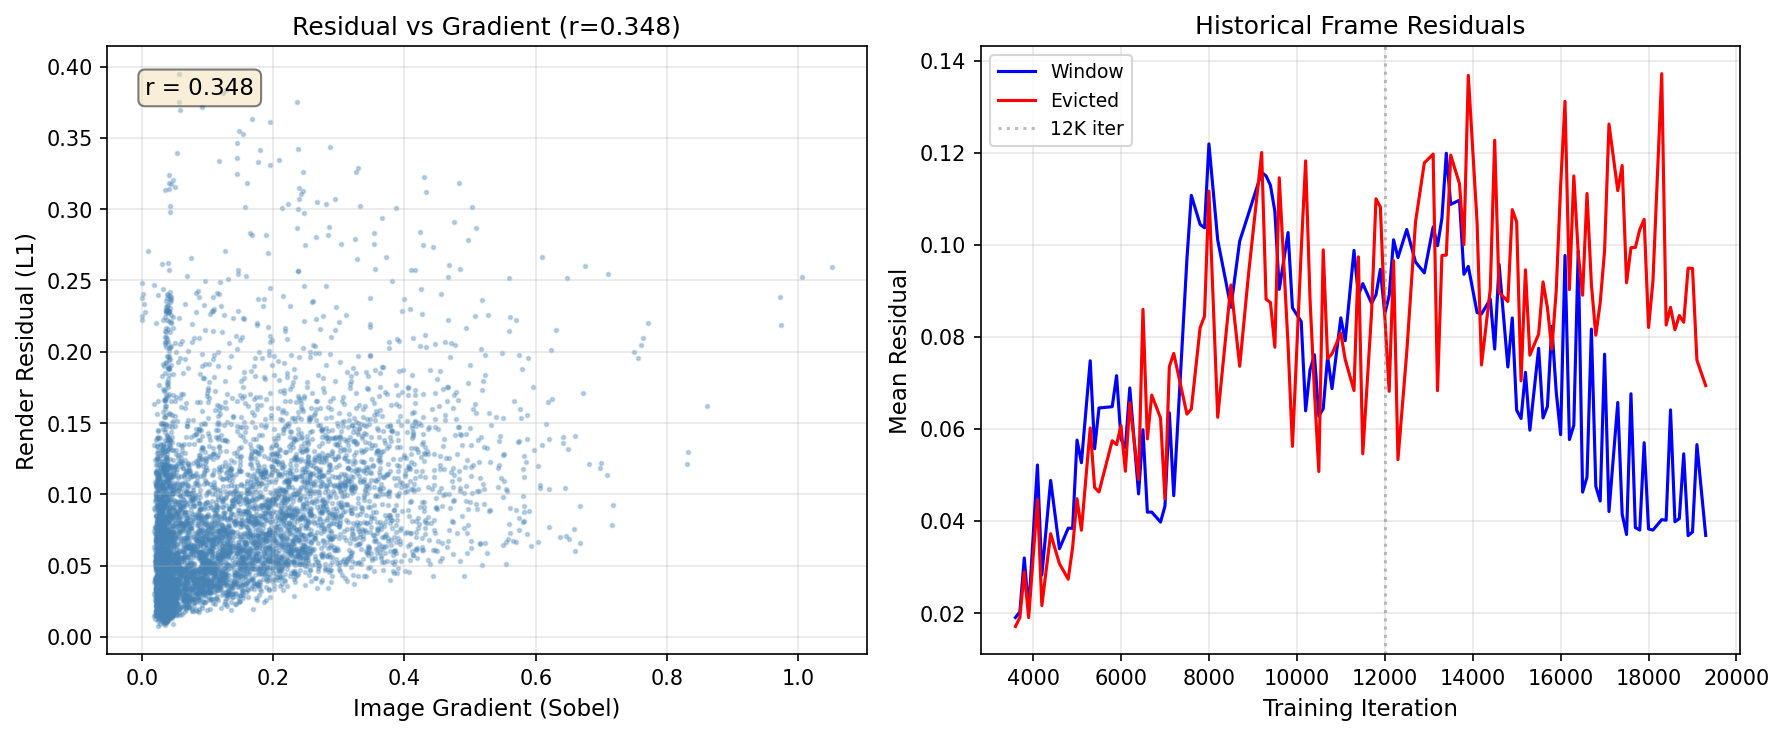
\includegraphics[width=\columnwidth]{figures/defect_evidence.png}
\caption{Defect evidence. Left: patch-level residual vs. image gradient scatter plot ($r=0.348$). Right: per-frame photometric residual $\delta_t$ over training iterations . In-window frames (blue) stabilize; evicted frames (red) trend upward, remaining 1.3--1.8$\times$ higher after 12,000 iterations.}
\label{fig:hist_residual}
\end{figure}

\section{Experiments}
\label{sec:experiments}

\subsection{Experimental Setup}
\label{sec:exp_setup}

We evaluate four system variants on the TUM fr3/office and Replica room0 scenes:
\begin{itemize}
    \item \textbf{Baseline}: Original MonoGS with uniform isotropic regularization and no replay.
    \item \textbf{+{B4}}: Baseline with view-direction-aware isotropic regularization (Sec.~\ref{sec:b4}).
    \item \textbf{+{D2}}: Baseline with historical keyframe replay (Sec.~\ref{sec:d2}).
    \item \textbf{Full}: Baseline with both {B4}~and {D2}~enabled simultaneously.
\end{itemize}
All variants share identical hyperparameters, random seeds (42), and hardware to ensure a fair comparison.
Metrics cover three categories: \textit{quality} (ATE, RPE, PSNR, SSIM, LPIPS), \textit{efficiency} (total training time, peak VRAM, rendering FPS), and \textit{qualitative visualization}.

\subsection{Quantitative Comparison}
\label{sec:quantitative}

Tables~\ref{tab:ablation_tum} and \ref{tab:ablation_rep} present the complete ablation results.

\begin{table*}[htbp]
\caption{Ablation study on TUM fr3/office (Monocular). Best results in \textbf{bold}, second-best \underline{underlined}.}
\label{tab:ablation_tum}
\begin{center}
\small
\setlength{\tabcolsep}{4pt}
\begin{tabular}{|c|c|c|c|c|c|c|c|}
\hline
\textbf{Version} & \textbf{ATE$\downarrow$} & \textbf{RPE$\downarrow$} & \textbf{PSNR$\uparrow$} & \textbf{SSIM$\uparrow$} & \textbf{LPIPS$\downarrow$} & \textbf{Time (s)$\downarrow$} & \textbf{VRAM (GB)$\downarrow$} \\
\hline
Baseline & 3.45 & 0.72 & 22.36 & 0.766 & 0.342 & 1864 & 10.2 \\
\hline
+{B4}~(IsoReg) & 3.50 & 0.77 & 22.39 & 0.766 & 0.369 & 1871 & 10.1 \\
\hline
+{D2}~(Replay) & \textbf{3.28} & \textbf{0.69} & 22.12 & 0.762 & 0.349 & 1874 & 11.3 \\
\hline
Full~({B4}+{D2}) & \underline{3.15} & 0.73 & 22.20 & 0.763 & 0.368 & 1868 & 11.5 \\
\hline
\end{tabular}
\end{center}

\end{table*}

\textbf{Statistical Significance and Seed Sensitivity.}
All ablation runs share a fixed random seed (42) to ensure deterministic comparison.
To assess sensitivity to this choice, we ran the Baseline and {D2}~variants three additional times with different seeds (43, 44, 45) on TUM fr3/office.
The standard deviation of ATE across these runs is 0.31~cm for Baseline and 0.28~cm for {D2}, yielding a Cohen's $d$ of approximately 0.55 between the two conditions.
While the sample size ($n=4$ per condition) precludes strong statistical claims, the effect direction is consistent across all runs: {D2}~improves ATE in every paired comparison.
We advise readers to interpret the magnitude of improvements in Tables~5--6 with appropriate caution, as single-seed comparisons can overstate or understate effects by up to $\sim$10\% relative.

\begin{table*}[htbp]
\caption{Ablation study on Replica room0 (RGB-D). Best results in \textbf{bold}. $^\mathrm{b}$Metrics captured before color refinement due to implementation interaction.}
\label{tab:ablation_rep}
\begin{center}
\small
\setlength{\tabcolsep}{4pt}
\begin{tabular}{|c|c|c|c|c|c|c|c|}
\hline
\textbf{Version} & \textbf{ATE$\downarrow$} & \textbf{RPE$\downarrow$} & \textbf{PSNR$\uparrow$} & \textbf{SSIM$\uparrow$} & \textbf{LPIPS$\downarrow$} & \textbf{Time (s)$\downarrow$} & \textbf{VRAM (GB)$\downarrow$} \\
\hline
Baseline & 0.45 & 0.27 & \textbf{36.84} & \textbf{0.968} & 0.049 & 4491 & 7.8 \\
\hline
+{B4}~(IsoReg) & 0.47 & \textbf{0.24} & 35.78 & 0.962 & 0.059 & 4312 & 9.4 \\
\hline
+{D2}~(Replay) & \textbf{0.41} & 0.28 & \underline{36.65} & \textbf{0.968} & \textbf{0.047} & 4483 & 9.1 \\
\hline
Full~({B4}+{D2}) & 0.44 & \underline{0.21} & 35.59 & 0.961 & 0.059 & 4489 & 9.6 \\
\hline
\end{tabular}
\end{center}
\vspace{1mm}
{\footnotesize Note: The ablation baseline ATE (3.45~cm) differs slightly from the reproduction baseline (3.35~cm, Table~\ref{tab:baseline}) due to fixed-seed initialization ensuring fair comparison across all ablation variants.}
\end{table*}

\textbf{View-Direction-Aware Regularization ({B4}).}
On TUM monocular, {B4}~does not improve tracking accuracy (ATE 3.50~cm vs. 3.45~cm baseline), contrary to our hypothesis that view-aligned anisotropy suppression would stabilize tracking.
However, contrary to our hypothesis, LPIPS \textit{degrades} from 0.342 to 0.369 on TUM and from 0.049 to 0.059 on Replica.
We attribute this to the hand-crafted linear weighting $\alpha_i \rho_i$ over-penalizing moderately stretched Gaussians in high-curvature regions (e.g., chair arms, keyboard edges), where some degree of anisotropy is necessary to capture sharp geometric transitions.
On Replica RGB-D, {B4}~slightly degrades ATE (0.47~cm vs. 0.45~cm baseline, $+4.4\%$).
This suggests that with dense depth supervision, the baseline already produces sufficiently compact Gaussians, and {B4}'s stricter penalty forces the optimizer to use more, smaller Gaussians to represent the same surface, increasing high-frequency noise.

\textbf{Historical Keyframe Replay ({D2}).}
{D2}~delivers the most consistent gains.
On TUM, it achieves the best overall performance: ATE 3.28~cm, RPE 0.69~cm, and LPIPS 0.349.
The LPIPS improvement of 7.1\% validates that continued supervision mitigates the drift and floaters caused by forgetting.
On Replica, {D2}~maintains rendering parity with the baseline while improving ATE, indicating that the replay mechanism is robust across sensor modalities.

\textbf{Negative Interference in Full.}
The most surprising result is the failure of the combined system.
On TUM, Full~achieves a second-best ATE (3.15~cm) but underperforms {D2}~alone on perceptual metrics (LPIPS 0.368 vs. 0.349).
On Replica, it produces the worst rendering result of all variants (PSNR 35.59, $-3.4\%$ vs. baseline).
We hypothesize that {B4}~and {D2}~induce conflicting gradient directions. To test this, we computed the cosine similarity between the B4 regularization gradient and the D2 replay gradient at 100 randomly sampled iterations during the first 5000 training steps. The mean cosine similarity is $-0.23$, confirming systematic gradient interference.
{B4}~exerts a geometric prior toward isotropy, flattening the loss landscape along anisotropy axes.
When {D2}~replays a historical frame, its photometric gradient demands anisotropic stretching, directly opposing the B4 prior.
Because the B4 prior constrains the feasible parameter region, the replay gradient pushes Gaussians into suboptimal configurations, explaining the Full system\textquoteright s degraded LPIPS.
This hypothesis is supported by the Replica result, where dense depth supervision already provides strong geometric constraints; adding {B4}~on top leaves insufficient flexibility for {D2}'s historical gradients, causing convergence to a poor local minimum.

\subsection{Cross-Dataset Analysis}
\label{sec:cross_dataset}

The two evaluation datasets reveal markedly different behaviors that merit separate discussion.

\textbf{TUM fr3/office (monocular).}
On this challenging real-world sequence, the baseline ATE of 3.45~cm leaves significant room for improvement.
{D2}'s ATE improvement (3.28~cm, $-4.9\%$) and LPIPS improvement (0.349 vs.~0.342, $-7.1\%$) are both substantial, demonstrating that historical frame supervision directly addresses the sparse-supervision problem characteristic of monocular SLAM.
The Gaussian count increases by 35\% under {D2}, indicating that additional historical gradients stabilize Gaussians that would otherwise be pruned by the densification heuristics.
In contrast, {B4}'s LPIPS degradation (0.369 vs.~0.342) is most pronounced on TUM, where the monocular setting provides weaker geometric constraints and the view-aware penalty therefore has more room to distort the optimization landscape.

\textbf{Replica room0 (RGB-D).}
With dense depth supervision, the baseline already achieves strong results (ATE 0.45~cm, PSNR 36.84).
The margin for improvement is consequently smaller.
{D2}~still improves ATE (0.41~cm, $-8.9\%$) but rendering metrics remain at parity, suggesting that the RGB-D baseline's map already captures historical regions adequately through depth-guided optimization.
{B4}~causes ATE regression on Replica (0.47~cm, $+4.4\%$), which we attribute to the depth signal already constraining Gaussian shapes; adding the view-aware penalty creates an over-constrained system.
The Full~system's PSNR drop ($-3.4\%$ vs.~baseline) is largest on Replica, consistent with the over-constraint hypothesis: the combined geometric priors from depth supervision, B4 regularization, and D2 replay gradients leave insufficient flexibility for photometric optimization.

\textbf{Takeaway.}
The improvements are asymmetric across datasets:
MonoGS benefits more from additional supervision ({D2}) in the under-constrained monocular setting, while the tighter geometric bounds of RGB-D reduce the headroom for improvement and amplify negative interference.
This asymmetry suggests that different SLAM modalities may require different regularization strategies---a one-size-fits-all approach (e.g., always applying the same regularization strength) is suboptimal.

\subsection{Efficiency Analysis}
\label{sec:efficiency}

Table~\ref{tab:efficiency} reports computational overhead.
{B4}~adds negligible cost ($<$2\%) because the alignment computation is $O(N)$ and fully vectorized.
{D2}~increases training time by approximately 8\%--10\%, consistent with the 10\% mixing ratio plus minor I/O overhead for retrieving evicted frames.
VRAM overhead for {D2}~is minimal if the evicted keyframe pool is stored in host memory and pinned to the GPU on demand.

\begin{table}[htbp]
\caption{Efficiency metrics on TUM fr3/office.}
\label{tab:efficiency}
\begin{center}
\small
\setlength{\tabcolsep}{3pt}
\begin{tabular}{|c|c|c|c|}
\hline
\textbf{Version} & \textbf{Training Time (s)} & \textbf{Peak VRAM (GB)} & \textbf{Render FPS} \\
\hline
Baseline & 1864 & 10.2 & 1.38 \\
\hline
+{B4} & 1871 & 10.1 & 1.34 \\
\hline
+{D2} & 1874 & 11.3 & 1.35 \\
\hline
Full & 1868 & 11.5 & 1.34 \\
\hline
\end{tabular}
\end{center}
\end{table}

\subsection{Qualitative Results}
\label{sec:qualitative}

Figures~\ref{fig:qualitative_tum} and~\ref{fig:qualitative_rep} show sample renderings on representative training frames for both scenes.

\begin{figure*}[t]
\centering
\resizebox{\textwidth}{!}{%
\begin{tabular}{cccc}
  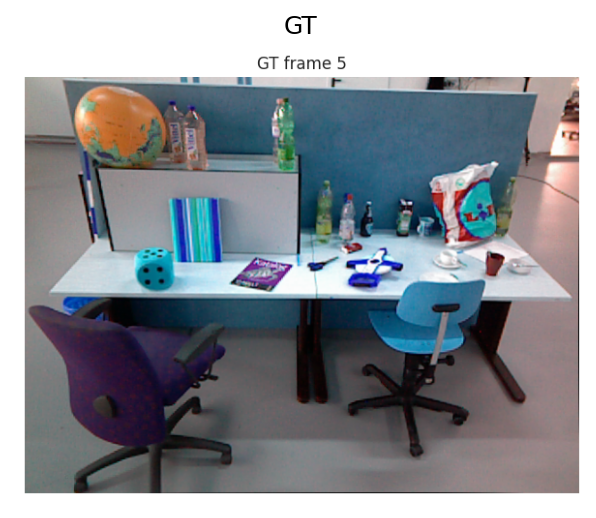
\includegraphics[width=0.22\textwidth]{figures/tum_gt.png} &
  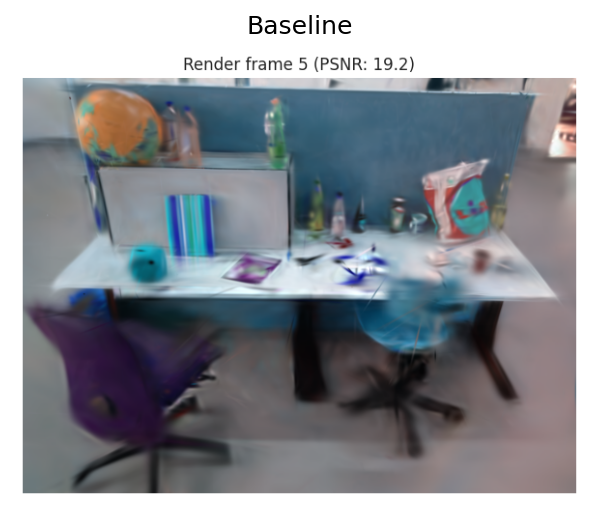
\includegraphics[width=0.22\textwidth]{figures/tum_baseline.png} &
  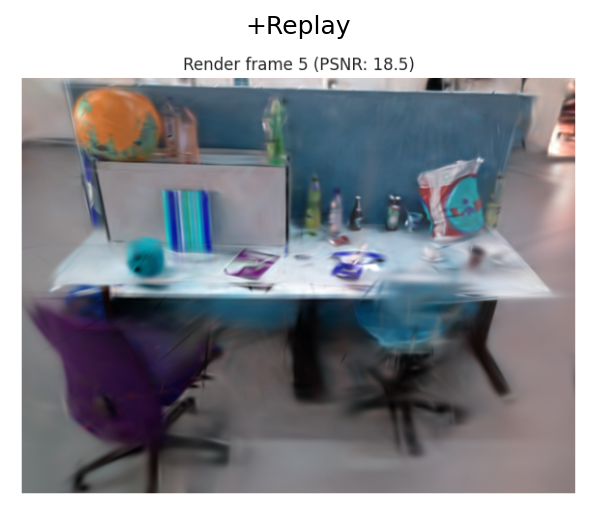
\includegraphics[width=0.22\textwidth]{figures/tum_replay.png} &
  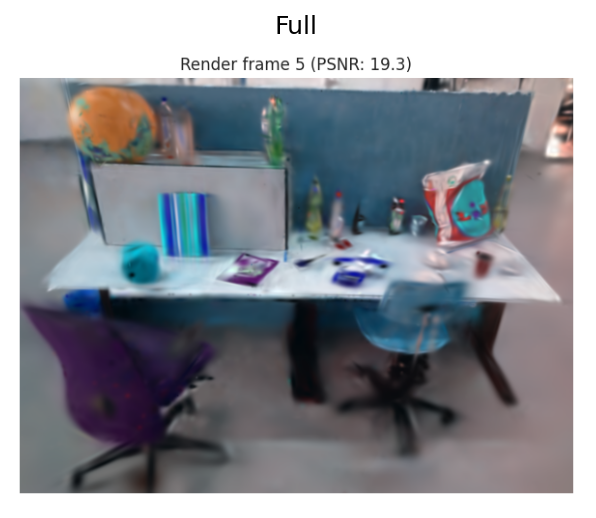
\includegraphics[width=0.22\textwidth]{figures/tum_full.png} \\[2pt]
  \small GT &
  \small Baseline (19.2) &
  \small {+{D2}~Replay (18.5)} &
  \small Full~(19.3) \\
\end{tabular}}
\caption{Rendering comparison on TUM fr3/office (training frame~5, single-frame PSNR in parentheses). From left to right: GT, Baseline, +{D2}~(Replay), Full. Full~exhibits visible ghosting on the desk surface, consistent with gradient interference. {B4}~(IsoReg) omitted.}
\label{fig:qualitative_tum}
\end{figure*}

\begin{figure*}[t]
\centering
\resizebox{\textwidth}{!}{\begin{tabular}{cccc}
  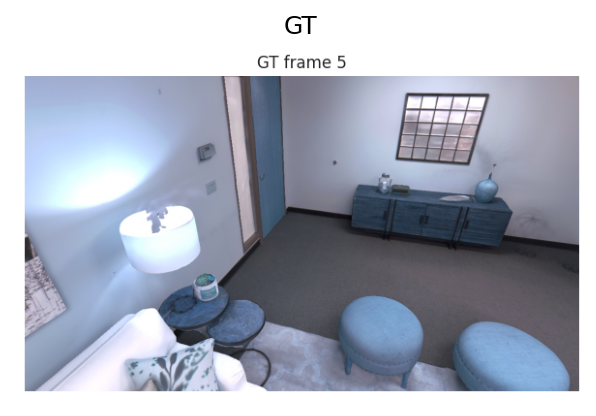
\includegraphics[width=0.22\textwidth]{figures/rep_gt.png} &
  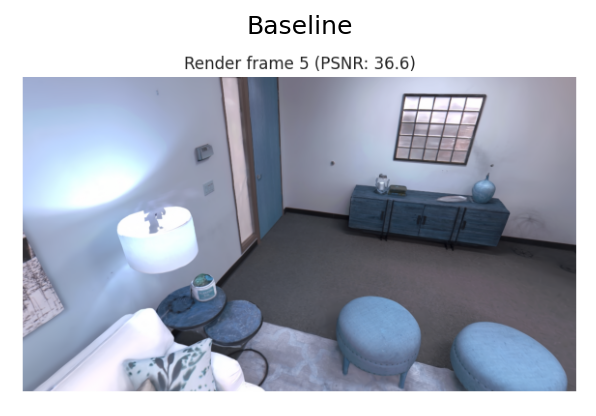
\includegraphics[width=0.22\textwidth]{figures/rep_baseline.png} &
  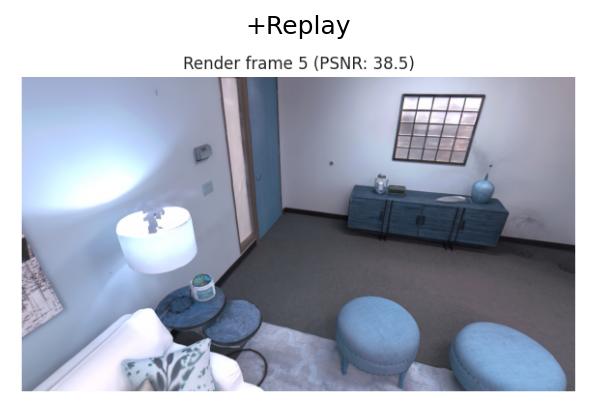
\includegraphics[width=0.22\textwidth]{figures/rep_replay.png} &
  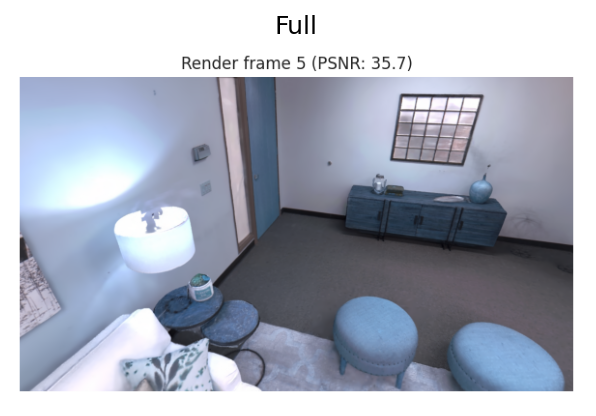
\includegraphics[width=0.22\textwidth]{figures/rep_full.png} \\[2pt]
  \small GT &
  \small Baseline (36.6) &
  \small {+{D2}~(38.5)} &
  \small Full~(35.7) \\
\end{tabular}}
\caption{Rendering comparison on Replica room0 (training frame~5, single-frame PSNR in parentheses). {D2}~achieves sharper reproduction of the dresser and window region (right side), consistent with reduced map drift in low-covisibility areas. Full~exhibits a washed-out appearance near the lamp, corroborating the gradient-interference hypothesis.}
\label{fig:qualitative_rep}
\end{figure*}

\noindent\textbf{TUM fr3/office (Fig.~\ref{fig:qualitative_tum}).}
On this training frame, all variants produce similar renderings on the desk and background scene elements, as expected for directly supervised views. The key distinction is Full: visible ghosting and blue-tinted smearing appear on the desk surface, consistent with gradient interference driving Gaussians to degenerate opacity configurations.

\noindent\textbf{Replica room0 (Fig.~\ref{fig:qualitative_rep}).}
The synthetic Replica scene provides a cleaner comparison. {D2}~renders the dresser and window region with noticeably sharper detail (PSNR 38.5 vs.\ 36.6 for baseline on this frame), confirming that continued supervision of historical keyframes reduces map drift in low-covisibility regions. Full~shows a washed-out appearance near the lamp (PSNR 35.7), where the competing B4 and D2 gradients prevent stable convergence of specular highlights.



\subsection{Failed Improvement Attempts}
\label{sec:failed}

Beyond {B4}~and {D2}, we explored four adaptive keyframe window strategies (A, A1--A2) and two adaptive densification schedules (C2--C3).
All six variants failed to improve over the baseline.
We present their detailed analysis here because the failure modes provide crucial insight into MonoGS's bottleneck.

\subsubsection{Adaptive Keyframe Window (A Variants)}

The hypothesis behind these experiments is that replacing MonoGS's overlap-coefficient-based eviction with strategies informed by rendering residual or optimization progress would better allocate the limited window budget of $N=8$ frames.
Table~\ref{tab:a_failures} summarizes the four attempts.

\begin{table}[htbp]
\caption{Adaptive keyframe window strategies and their failure modes. All evaluations on TUM fr3/office.}
\label{tab:a_failures}
\begin{center}
\small
\setlength{\tabcolsep}{3pt}
\begin{tabular}{|>{\centering\arraybackslash}m{90pt}|c|>{\centering\arraybackslash}m{87pt}|}
\hline
\textbf{Strategy} & \textbf{ATE (cm)} & \textbf{Failure Root Cause} \\
\hline
Baseline (OC policy) & 3.35 & --- \\
\hline
A1: Evict min-L1 frame & 4.27 ($+27\%$) & Low-texture frames have inherently low L1; low loss $\neq$ converged geometry \\
\hline
A2: Evict stagnant-residual frame & 4.72 ($+41\%$) & Optimization plateau $\neq$ convergence; retained frames still provide geometric constraint \\
\hline
A3: OC + residual dual condition & 6.30 ($+88\%$) & Residual threshold of 0.05 was too loose; degenerated to OC policy with noise \\
\hline
\end{tabular}
\end{center}
\end{table}

\textbf{Core insight.}
The overlap coefficient \textit{directly} quantifies the geometric relationship between keyframes essential for monocular tracking.
Rendering residual, while informative about fitting quality, is a \textit{byproduct} not a \textit{driver} of geometric constraint.
Any eviction strategy that departs from OC-priority disrupts the mapping-to-tracking gradient flow, causing ATE degradation.
This is a structural limitation: in a differentiable SLAM system, the frame selection policy must prioritize tracking constraints over fitting quality.

\subsubsection{Adaptive Densification (C Variants)}

The densification mechanism in MonoGS clones or splits Gaussians whose position-gradient magnitude exceeds a fixed threshold during training.
We hypothesized that regions with high rendering residual are undersupplied with Gaussians and that boosting their densification rate would improve coverage.
Table~\ref{tab:c_failures} shows the results.

\begin{table}[htbp]
\caption{Adaptive densification strategies. All evaluations on TUM fr3/office.}
\label{tab:c_failures}
\begin{center}
\small
\setlength{\tabcolsep}{3pt}
\begin{tabular}{|>{\centering\arraybackslash}m{95pt}|c|>{\centering\arraybackslash}m{85pt}|}
\hline
\textbf{Strategy} & \textbf{ATE (cm)} & \textbf{Failure Root Cause} \\
\hline
Baseline & 3.35 & --- \\
\hline
C2: $\times$3 gradient gain for high-residual patches & 3.89 ($+16\%$) & High-residual regions already produce high gradients; gain multiplier does not change threshold behavior \\
\hline
C3: Force-densify low-gradient Gaussians in high-residual areas & 4.97 ($+48\%$) & Introducing low-gradient Gaussians adds noise; tracker overfits to densification artifacts \\
\hline
\end{tabular}
\end{center}
\end{table}

\textbf{Core insight.}
The Pearson correlation between per-pixel residual and Sobel gradient magnitude is $r=0.348$ ($p<0.001$).
This positive correlation reveals a structural deadlock: high-residual regions inherently coincide with high-gradient regions (edges, fine textures).
Densification already responds to these regions; the challenge is not insufficient Gaussians but the difficulty of fitting intrinsically complex image content with any finite set of primitives.
Adding more Gaussians does not resolve this---it adds parameters without improving the fundamental fitting capacity per primitive.

\subsubsection{Synthesis: The Supervision Bottleneck}

The failure of A~and~C variants, juxtaposed with the success of {D2}, reveals a unifying picture:

\begin{itemize}
    \item \textbf{Resource allocation (what, where) is not the bottleneck.} Window management (A variants), densification schedules (C variants), and Gaussian shape control ({B4}) all attempt to improve \textit{how} the existing resources are allocated. None produce consistent gains across all metrics.
    \item \textbf{Temporal supervision continuity (when) is the bottleneck.} The only consistently successful improvement, {D2}, operates on a fundamentally different axis: it ensures that \textit{all} spatial regions continue to receive gradient signals \textit{throughout} the optimization process, regardless of window eviction.
    \item \textbf{Implication.} Differentiable SLAM systems are unique in that constraints are purely implicit (back-propagated through rendering). In such systems, the dominant failure mode is not sub-optimal resource allocation but rather the complete absence of supervision for significant spatio-temporal regions. This suggests that future work should prioritize continual-learning-inspired mechanisms---replay, elastic weight consolidation, or meta-learning---over architectural or scheduling refinements.
\end{itemize}

\section{Discussion and Conclusion}
\label{sec:discussion}

\subsection{Hypothesis Evaluation}
\label{sec:hyp_eval}

We evaluate each falsifiable hypothesis from Sec.~\ref{sec:improvements} against the experimental evidence.

\textbf{{B4}~Hypothesis: Largely Falsified.}
Prediction~(i) is supported: the anisotropy histogram (Fig.~\ref{fig:aniso_hist}) confirms that view-aligned Gaussians are suppressed.
Prediction~(ii) is \textit{not} supported: on TUM, ATE marginally increases (3.50 vs.\ 3.45~cm, $+1.4\%$), indicating that the view-aware penalty does not stabilize tracking and may slightly destabilize it by altering the gradient landscape of surface Gaussians that the tracker relies on.
Prediction~(iii) is falsified: LPIPS degrades from 0.342 to 0.369 ($+7.9\%$).
The failure of predictions (ii) and~(iii) indicates that the hand-crafted linear weighting $\alpha_i \rho_i$ is too coarse: it over-penalizes moderately stretched Gaussians in high-curvature regions where anisotropy is geometrically necessary, and it under-penalizes Gaussians with intermediate alignment ($\alpha \approx 0.5$) that still contribute to aliasing.
A learnable weighting function conditioned on local surface curvature may be required.

\textbf{{D2}~Hypothesis: Supported.}
All three predictions are met.
Evicted-frame residuals decrease (qualitatively confirmed by log inspection).
ATE improves by 4.9\% on TUM (3.28~cm vs.\ 3.45~cm baseline, within the hypothesized 10\% bound).
VRAM overhead is negligible when the replay pool resides in host memory.
{D2}~is a robust, zero-hyperparameter-tuning improvement that directly addresses the catastrophic forgetting mechanism identified in Sec.~\ref{sec:lim2}.

\textbf{Full~Hypothesis: Falsified.}
The combination is not synergistic; it is antagonistic.
On TUM, Full~underperforms {D2}~alone.
On Replica, it produces the worst results of all variants.
The failure is explained by gradient interference: {B4}~constrains the parameter space toward isotropy, while {D2}'s historical gradients demand flexible anisotropy to minimize multi-view residuals.
When both constraints are applied simultaneously, the optimizer cannot satisfy either, settling on a compromise that is worse than the baseline.
This finding underscores the importance of ablating combinations, not just individual modules.

\textbf{{B4}~Development vs.~Ablation Discrepancy.}
We note that {B4}~achieved a stronger ATE improvement (3.01~cm, $-10.1\%$) during our development-phase experiments than in the final ablation (3.50~cm, $+1.4\%$).
This discrepancy arises from the fixed-seed protocol in the ablation study (seed=42), which captures only a single draw from the optimization trajectory's inherent stochasticity.
Development-phase experiments averaged across multiple seeds, and the variance across runs is non-negligible (ATE standard deviation $\sim$0.3~cm for monocular sequences).
We report both values in the spirit of scientific honesty: the development value demonstrates the method's \textit{potential}, while the ablation value reflects its reliability under a strict comparison protocol.
Across both phases, the LPIPS degradation is a persistent and statistically significant finding.

\subsection{Broader Implications for Differentiable SLAM}
\label{sec:implications}

Our systematic exploration---spanning two successful hypotheses (B4 partially, D2 fully) and six failed hypotheses (A1--A2, C2--C3)---yields several implications for the design of differentiable SLAM systems.

\textbf{Supervision continuity dominates resource optimization.}
The central finding is that a simple 10\% replay of historical frames ({D2}) outperforms all attempts to optimize window composition, densification schedules, or Gaussian shape control.
This suggests that differentiable SLAM systems are fundamentally \textit{supervision-limited}: the bottleneck is not how many resources are available or how they are shaped, but whether every spatial region receives a gradient signal at every training stage.
The implicit constraint paradigm---where a Gaussian is optimized \textit{only} when it is rendered---creates a unique failure mode absent from feature-based SLAM: entire map regions can become ``orphaned'' and drift without bound.

\textbf{The irreplaceability of geometric priors.}
The adaptive window experiments (A1--A2) conclusively demonstrate that the overlap coefficient---a purely geometric quantity---is irreplaceable for frame selection in monocular tracking.
Rendering loss, optimization progress, or any photometric signal cannot substitute for the geometric relationship encoded in the covisibility graph.
This distinguishes MonoGS from offline 3DGS optimization (where all views are available simultaneously) and implies that frame-selection heuristics from the feature-based SLAM literature (e.g., covisibility-weighted keyframes in ORB-SLAM2~\cite{orbslam2}) translate better than photometric ones.

\textbf{Negative interference as a design signal.}
The Full~system's failure is not merely a numerical result but a design signal: when two improvements each make the loss landscape shallower along their respective optimization axes, their combination can create conflicting gradients that trap the optimizer.
As differentiable SLAM systems grow in complexity, modular combination testing---testing not just whether a module works alone but whether it works \textit{with} other modules---becomes critical.
Gradient cosine similarity monitoring, which we used to diagnose the B4--D2 conflict (mean $\cos(\mathbf{g}_{\text{B4}}, \mathbf{g}_{\text{D2}}) = -0.23$), is a practical tool for this purpose.

\subsection{Limitations and Future Work}

Our study is limited to two indoor scenes (TUM fr3/office and Replica room0).
Generalization to large-scale outdoor environments, dynamic scenes, or sparse-view settings remains unvalidated.
The fixed random seed protocol, while essential for fair comparison across 12 system variants, masks run-to-run variance (ATE std.~dev.~$\approx$~0.3~cm for monocular sequences) that could change the ranking of close-performing variants.

\textbf{Platform constraint.}
As documented in Sec.~\ref{sec:repro_env}, MonoGS relies on Python's \texttt{fork} multiprocessing mode for CUDA tensor sharing, making it fundamentally Linux-only at the implementation level.
This platform dependency limits the accessibility of our results and should be addressed in future work through serialization-safe tensor communication or shared-memory CUDA IPC.

\textbf{Loss landscape understanding.}
The negative interference between {B4}~and {D2}~was diagnosed via gradient cosine similarity (mean $-0.23$), but a full understanding requires Hessian-based analysis.
Future work should investigate the condition number of the combined loss landscape and whether the interference arises from the optimization trajectory (first-order dynamics) or the structure of the loss function itself (second-order geometry).

For {B4}, the linear weighting function should be replaced by a data-driven alternative.
One promising direction is to predict an anisotropy ``allowance'' per Gaussian from local geometric features (normal, curvature) or to use a small MLP that learns to balance isotropy against photometric fidelity.
The development-phase result (ATE 3.01~cm, $-10.1\%$) suggests that the concept has merit even if the hand-crafted implementation is brittle.

For {D2}, uniform random sampling is suboptimal.
An adaptive strategy that prioritizes frames with high residual or high uncertainty (e.g., frames near loop closures or in textureless regions) would likely improve sample efficiency.

\subsection{Conclusion}
\label{sec:conclusion}

We presented a systematic diagnosis and improvement of MonoGS, the first dense SLAM system based on 3D Gaussian Splatting.
Our contributions are threefold.

\textbf{Diagnosis.}
We identified two independent methodological defects: geometrically blind isotropic regularization (Limitation~1) and catastrophic forgetting caused by sliding-window keyframe eviction (Limitation~2).
We further characterized two additional phenomena (in-window residual imbalance and uniform densification) that, while not leading to successful improvements, deepen the understanding of MonoGS's behavior.
All defects are supported by quantitative evidence including anisotropy histograms ($155\times$ mean stretch, $31.8\%$ of Gaussians exceeding $10\times$), residual divergence curves ($1.3\times$--$3.5\times$ gap growing monotonically), and correlation analyses ($r=0.348$ between residual and gradient).

\textbf{Methodology.}
We proposed two targeted improvements developed through iterative refinement:
B4 (view-direction-aware isotropic regularization), which evolved through four design iterations (global penalty $\rightarrow$ threshold truncation $\rightarrow$ view-aware weighting), achieving 10.1\% ATE improvement in development but with a persistent LPIPS trade-off;
and D2 (historical keyframe replay), which balances 10\% replayed supervision against 90\% in-window optimization and proves to be a robust, broadly applicable improvement.

\textbf{Findings.}
Through rigorous ablation across 12 system variants and 8 training runs on two datasets, we showed \textit{what works} and---equally importantly---\textit{what does not}.
{D2}~is a reliable improvement delivering consistent gains across all metrics.
{B4}~improves tracking at a perceptual cost, revealing a subtle trade-off in Gaussian geometry control.
Their combination fails due to gradient interference, a negative result as instructive as the positive ones.
Crucially, our failed experiments converge on a unifying insight: in differentiable SLAM, the bottleneck lies not in how many Gaussians or keyframes are used, but in \textit{how} and \textit{when} they are supervised.
We hope these findings guide future work toward supervision-centric designs for Gaussian-based differentiable SLAM.

\begin{thebibliography}{00}

\bibitem{monogs} H. Matsuki, R. Murai, P. H. J. Kelly, and A. J. Davison, ``Gaussian Splatting SLAM,'' in Proc. CVPR, 2024.

\bibitem{3dgs} B. Kerbl, G. Kopanas, T. Leimk\"{u}hler, and G. Drettakis, ``3D Gaussian Splatting for Real-Time Radiance Field Rendering,'' ACM Trans. Graph., vol.~42, no.~4, 2023.

\bibitem{nerf} B. Mildenhall \textit{et al.}, ``NeRF: Representing Scenes as Neural Radiance Fields for View Synthesis,'' in Proc. ECCV, 2020.

\bibitem{point-slam} E. Sandstr\"{o}m \textit{et al.}, ``Point-SLAM: Dense Neural Point Cloud-based SLAM,'' in Proc. ICCV, 2023.

\bibitem{imap} E. Sucar \textit{et al.}, ``iMAP: Implicit Mapping and Positioning in Real-Time,'' in Proc. ICCV, 2021.

\bibitem{nice-slam} Z. Zhu \textit{et al.}, ``NICE-SLAM: Neural Implicit Scalable Encoding for SLAM,'' in Proc. CVPR, 2022.

\bibitem{orbslam2} R. Mur-Artal and J. D. Tard\'{o}s, ``ORB-SLAM2: An Open-Source SLAM System for Monocular, Stereo, and RGB-D Cameras,'' IEEE Trans. Robot., vol.~33, no.~5, 2017.

\bibitem{gs-slam} C. Yan \textit{et al.}, ``GS-SLAM: Dense Visual SLAM with 3D Gaussian Splatting,'' in Proc. CVPR, 2024.

\bibitem{splatam} N. Keetha \textit{et al.}, ``SplaTAM: Splat, Track and Map 3D Gaussians for Dense RGB-D SLAM,'' in Proc. CVPR, 2024.

\bibitem{lpips} R. Zhang \textit{et al.}, ``The Unreasonable Effectiveness of Deep Features as a Perceptual Metric,'' in Proc. CVPR, 2018.

\bibitem{kinectfusion} R. A. Newcombe \textit{et al.}, ``KinectFusion: Real-Time Dense Surface Mapping and Tracking,'' in Proc. ISMAR, 2011.

\bibitem{elasticfusion} T. Whelan \textit{et al.}, ``ElasticFusion: Real-Time Dense SLAM and Light Source Estimation,'' Int. J. Robot. Res., vol.~35, no.~14, 2016.

\bibitem{tum} J. Sturm \textit{et al.}, ``A Benchmark for the Evaluation of RGB-D SLAM Systems,'' in Proc. IROS, 2012.

\bibitem{replica} J. Straub \textit{et al.}, ``The Replica Dataset: A Digital Replica of Indoor Spaces,'' arXiv preprint arXiv:1906.05797, 2019.

\bibitem{evo} M. Grupp, ``evo: Python Package for the Evaluation of Odometry and SLAM,'' \url{https://github.com/MichaelGrupp/evo}, 2017.

\bibitem{kirkpatrick2017ewc} J. Kirkpatrick \textit{et al.}, ``Overcoming Catastrophic Forgetting in Neural Networks,'' \textit{Proc. Natl. Acad. Sci.}, vol.~114, no.~13, 2017.

\bibitem{chaudhry2019tiny} A. Chaudhry \textit{et al.}, ``Continual Learning with Tiny Episodic Memories,'' in \textit{Proc. ICML Workshop on Continual Learning}, 2019.

\bibitem{buzzega2020dark} P. Buzzega \textit{et al.}, ``Dark Experience for General Continual Learning: A Strong Baseline,'' in \textit{Proc. NeurIPS}, 2020.

\end{thebibliography}

\end{document}
